\documentclass[UTF8]{ctexart}
\CTEXsetup[format={\Large\bfseries}]{section}
\setCJKmainfont{KaiTi}
\setmainfont{Times New Roman}
\usepackage{geometry}
\geometry{a4paper, left=3.4cm, right=3.4cm, top=2.4cm, bottom=2.4cm}
%\geometry{a4paper, scale=0.75}
%\usepackage{setspace}
%\onehalfspacing
\addtolength{\parskip}{-0.1em}
\usepackage{amsmath}
\usepackage{graphicx}
\usepackage{float}
\usepackage{subfigure}
\usepackage{fancyhdr}
\pagestyle{plain}
\usepackage{caption}
\renewcommand{\figurename}{Figure}
\usepackage[colorlinks,linkcolor=blue,anchorcolor=blue, citecolor=blue, bookmarks, bookmarksopen, pdfstartview=FitH]{hyperref} 
\usepackage{listings}
\usepackage{xcolor}
\usepackage{fontspec}
\usepackage{algorithm}
\usepackage{algorithmicx}
\usepackage{algpseudocode}
\lstset{
	numbers=left, 
	numberstyle= \tiny, 
	basicstyle=\fontspec{Consolas},
	keywordstyle=\color{ blue!70},
	commentstyle={
		\color{red!50!green!50!blue!50} \fontspec{Consolas Italic}},
	frame=shadowbox,
	rulesepcolor= \color{ red!20!green!20!blue!20},
	escapeinside=``,
	xleftmargin=2em,xrightmargin=2em, aboveskip=1em,
	framexleftmargin=2em,
} 

\makeatletter
\newenvironment{breakablealgorithm}
{% \begin{breakablealgorithm}
	\begin{center}
		\refstepcounter{algorithm}% New algorithm
		\hrule height.8pt depth0pt \kern2pt% \@fs@pre for \@fs@ruled
		\renewcommand{\caption}[2][\relax]{% Make a new \caption
			{\raggedright\textbf{\ALG@name~\thealgorithm} ##2\par}%
			\ifx\relax##1\relax % #1 is \relax
			\addcontentsline{loa}{algorithm}{\protect\numberline{\thealgorithm}##2}%
			\else % #1 is not \relax
			\addcontentsline{loa}{algorithm}{\protect\numberline{\thealgorithm}##1}%
			\fi
			\kern2pt\hrule\kern2pt
		}
	}{% \end{breakablealgorithm}
		\kern2pt\hrule\relax% \@fs@post for \@fs@ruled
	\end{center}
}
\makeatother

\title{Image Warping\footnote{https://github.com/sdc17/NaiveIW}} 
\author{石大川\quad <sdc17@mails.tsinghua.edu.cn>}
\date{\today}
\begin{document}
	\maketitle
%	\tableofcontents \newpage
	\section*{Affine Warping}
	因为在实验中发现Affine Warping不能完美贴合边界,所以实际做的是Projective Warping.
	\subsection*{Procedure}
	\begin{algorithm}[h]
		\caption{Projective Warping}
		\begin{algorithmic}[1]
			\State 选定投影结果的四个顶点
			\For{每个选中的顶点}
			\State 根据如下矩阵得到关于$x'$和$y'$的两个方程
			\begin{equation*}
				\begin{bmatrix} x' \\ y' \\ w'\end{bmatrix} = 
				\begin{bmatrix} a&b&c \\ d&e&f \\ g&h&1 \end{bmatrix}
				\begin{bmatrix} x \\ y \\ w \end{bmatrix}
			\end{equation*}	
			\EndFor
			\State $fsolve$解方程组得到八个系数的值
			\ForAll{$pixel\in source.jpg$}
			\State 根据如下方程算出对应$target.jpg$中的位置并做相应的投影
			\begin{equation*}
				x'= \frac{ax+by+cw}{gx+hy+w} 
			\end{equation*}
			\begin{equation*}
				y' = \frac{dx+ey+fw}{gx+hy+w}
			\end{equation*}
			\EndFor
		\end{algorithmic}
	\end{algorithm}
	Affine Warping相比Projective Warping的流程只是将系数$g$和$h$简化为了$0$
	\subsection*{Result}
	
	\hyperref[Fig.projective]{Figure 1}展示了实验结果, 其中\hyperref[Fig.sub.1]{Figure a}是以红圈标出的三个顶点为目标做的Affine Warping, 可见在蓝框标出的第四个顶点附近贴合程度并不好。 相对地,\hyperref[Fig.sub.2]{Figure b}是选定四个顶点做Projective Warping的结果,可见贴合程度是比较理想的。
	
	\begin{figure}[htbp]
		\centering 
		\subfigure[Affine Warping]{
			\label{Fig.sub.1}
			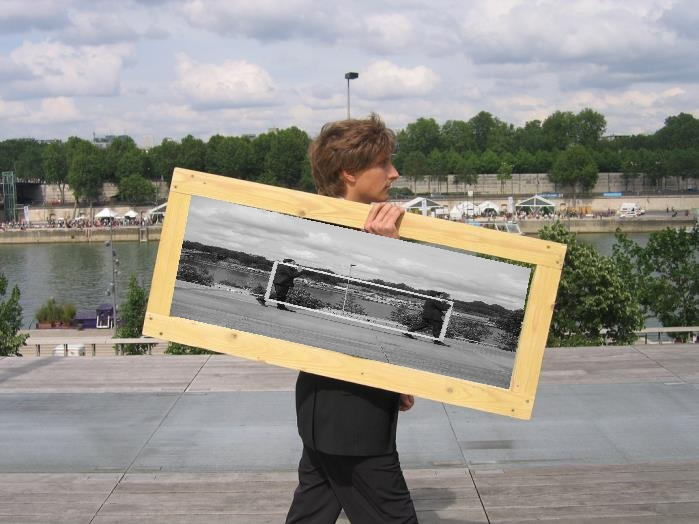
\includegraphics[width=0.45\textwidth]{affine.jpg}}
		\subfigure[Projective Warping]{
			\label{Fig.sub.2}
			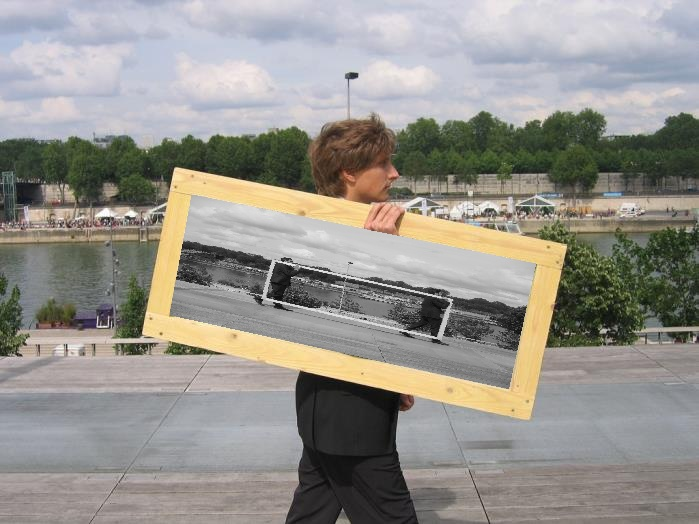
\includegraphics[width=0.45\textwidth]{projective.jpg}}
		\caption{Affine Warping and Projective Warping}
		\label{Fig.projective}
	\end{figure}
	
	\section*{Sphere Warping}
	因为给的原图比较糊,所以自己在网上找了同一张图的高清版本作为替代并且保留了原图$4:3$的长宽比。
	\subsection*{Procedure}\vspace{3ex}
	\begin{breakablealgorithm}
		\caption{Sphere Warping}
		\begin{algorithmic}[1]
			\State 分别计算输入输出的最大中心距离$d_0$和$\rho_0$
			\ForAll{$pixel\in sphere.jpg$}
			\State 对于输出图像中的每个像素点计算
			\begin{equation*}
			\rho = \sqrt{r_{out}^2+c_{out}^2}
			\end{equation*}
			\begin{equation*}
			\theta = tan^{-1}(\frac{r_{out}}{c_{out}})
			\end{equation*}
			\begin{equation*}
			\phi = sin^{-1}(\frac{\rho}{\rho_0})
			\end{equation*}
			\If {pixel到圆心的距离小于$\rho$}
			\State 根据如下公式得到原图中相应$pixel$偏离中心的距离
			\begin{equation*}
			d = \frac{2d_0\phi}{\pi}
			\end{equation*}
			\begin{equation*}
			r_{in}=dsin(\theta)
			\end{equation*}
			\begin{equation*}
			c_{in}=dcos(\theta)
			\end{equation*}
			\If {对应原图的$pixel$超出了原图尺寸范围}
			\State 输出的$pixel$置为$[127, 127, 127]$
			
			\Else
			\State 根据行偏移$r_{in}$和列偏移$c_{in}$得到原像素地址并做$Bilinear$
			\begin{equation*}
			f(x, y)=\frac{1}{(x_2-x_1)(y_2-y_1)}\begin{bmatrix} x_2-x&x-x_1\end{bmatrix}
			\begin{bmatrix} f(Q_{11})&f(Q_{12})\\ f(Q_{21})&f(Q_{22})\end{bmatrix}
			\begin{bmatrix} y_2-y \\ y-y_1\end{bmatrix}
			\end{equation*}
			\State 其中$Q_{11},Q_{21},Q_{22},Q_{12}$分别是从左下角开始沿逆时针方向的四个相邻整数坐标点的像素值
			\EndIf
			\EndIf
			\EndFor
		\end{algorithmic}
	\end{breakablealgorithm}
	
	\subsection*{Result}
	\hyperref[Fig.sphere]{Figure 2}展示了实验结果, 其中\hyperref[Fig.sub.3]{Figure a}的插值方法是直接使用距离最近的一个像素,\hyperref[Fig.sub.4]{Figure b}中用的是Bilinear插值。放大后对比可以发现在图像细节上,第二种插值方式是优于第一种插值方式的。例如对比左图红框标出的位置和右图中对应的位置可见,右图此处垂直方向的白色直线错位程度更低。
	
	\begin{figure}[htbp]
		\centering 
		\subfigure[Nearest Interpolation]{
			\label{Fig.sub.3}
			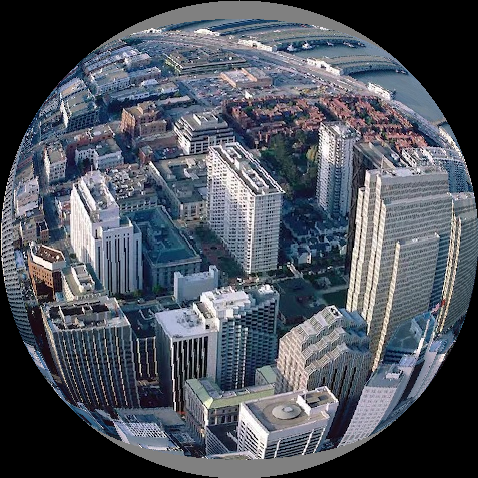
\includegraphics[width=0.45\textwidth]{sphere_without_bilinear.png}}
		\subfigure[Bilinear Interpolation]{
			\label{Fig.sub.4}
			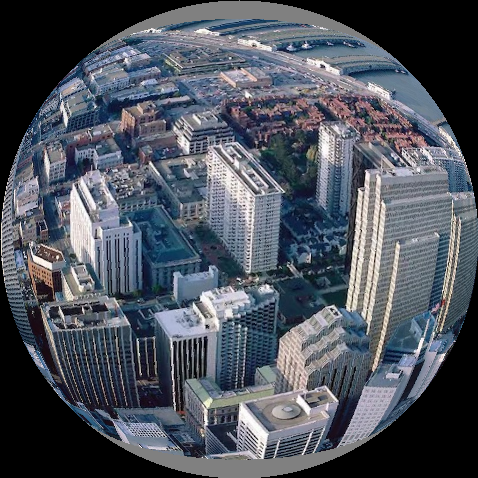
\includegraphics[width=0.45\textwidth]{sphere.png}}
		\caption{Sphere Warping}
		\label{Fig.sphere}
	\end{figure}
	
	\section*{Water Wave Warping}
	效果类似于在平静的湖面上扔一颗石子,然后以石子落点为中心湖面会泛开涟漪。
	
	\subsection*{Procedure}\vspace{3ex}
	\begin{breakablealgorithm}
		\caption{Water Wave Warping}
		\begin{algorithmic}[1]
			\State 选定一个在原图尺寸范围内的波动中心$center$
			\ForAll{$pixel\in ww.jpg$}
			\State 计算每个$pixel$到波动中心的相对位置
			\begin{equation*}
			x_{relative} = x_{origin} - center_{col}
			\end{equation*}
			\begin{equation*}
			y_{relative} = center_{row} - y_{origin}
			\end{equation*}
			\State 根据相对位置计算$pixel$到波动中心的夹角
			\begin{equation*}
			\theta = \arctan\frac{y_{relative}}{x_{relative}}
			\end{equation*}
			\State 计算波动前$pixel$到波动中心的距离
			\begin{equation*}
			r_{0} = \sqrt{x_{relative}^2 + y_{relative}^2}
			\end{equation*}
			\State 计算波动后$pixel$到波动中心的距离,其中$decay$和$velocity$分别是控制衰减和传播速度的超参数
			\begin{equation*}
			r = r_{0} + decay \times shape_{col} \times \sin(velocity \times r_{0})
			\end{equation*}
			\EndFor
			\State 根据波动后的距离转换到相应的$pixel$位置
			\begin{equation*}
			x_{out} = r \times \cos \theta + center_{col}
			\end{equation*}
			\begin{equation*}
			y_{out} = center_{row} - r \times \sin \theta
			\end{equation*}
			\ForAll{$pixel\in result.jpg$}
			\If{按照前述流程得到对应到原图中的像素位置没有超出原图尺寸}
			\State 按照已经计算出的映射关系,做$Bilinear$插值得到结果$pixel$
			\Else
			\State 第一行根据左边的$pixel$插值,第一列根据上边的$pixel$插值,其余的根据左上的$pixel$插值
			\EndIf
			\EndFor
		\end{algorithmic}
	\end{breakablealgorithm}
	
	\subsection*{Result}
	
	\hyperref[Fig.waterwave]{Figure 3}展示了实验结果, 其中\hyperref[Fig.sub.5]{Figure a}是原图,\hyperref[Fig.sub.6]{Figure b}是做Water Wave Warping后的结果。在观感上确实产生了水面涟漪的效果,在结果图中也能较容易地识别出原图的轮廓,这符合在实际生活中向水面投掷石子的结果。\\
	
	此外,更进一步还可以做多个波动的干涉结果,直观上类似于向水面不同位置投掷多枚石子。因为波动的干涉有线性叠加性,所以在每个像素点将来自不同地方的多个波叠加起来即可。
	\begin{figure}[htbp]
		\centering 
		\subfigure[Origin Photo]{
			\label{Fig.sub.5}
			\includegraphics[width=0.95\textwidth]{ww.jpg}}
		\subfigure[Result Photo]{
			\label{Fig.sub.6}
			\includegraphics[width=0.95\textwidth]{ww.png}}
		\caption{Sphere Warping}
		\label{Fig.waterwave}
	\end{figure}

	\section*{Conlusion}
	这次作业加深了我对于Image Warping和Bilinear等插值方式的理解,动手实现三种Image Warping和Bilinear插值方式的过程则让我对于numpy和scipy的使用变得更加熟练。
	
\end{document}